\chapter{Metodologia} 
\label{chap:metodologia}

O objetivo deste trabalho é propor e investigar uma arquitetura de aprendizado profundo que unifica características radiômicas e características profundas. Inicialmente, é empregado diversas técnicas de aprendizado de máquina para extrair características manuais de imagens de RM, abrangendo textura, forma, escala de cinza, etc. Posteriormente, uma rede \textit{ResNet50} pré-treinada é utilizada para extrair características profundas que encapsulam informações semânticas de alto nível e de representação das imagens de \gls{RMC}. Estas características são então fundidas em um vetor de características unificado. Para aprimorar a acurácia e a robustez, um módulo foi desenvolvido utilizando o mecanismo de autoatenção, módulo este que otimiza e pondera o vetor de características fundidas de forma eficaz. A Figura \ref{fig:fig015} confere o fluxograma do projeto ilustrando de forma esquemática as fases que serão atuadas.

\begin{figure}[h!]
    \centering
    \caption{Fluxograma do Projeto}
    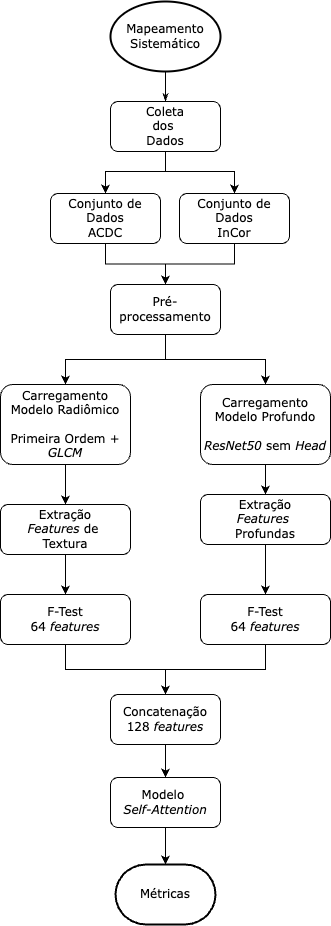
\includegraphics[width=0.4\textwidth]{figures/fig015.png}
    \caption*{Fonte: Autor}
    \label{fig:fig015}
\end{figure}

%--------------------------------------------------------
\section{Bases de Dados} 
\label{subsec:cap4_dataset}

Duas bases de dados serão utilizas para experimento. O primeiro conjunto de dados é o \gls{ACDC}\footnote{https://www.creatis.insa-lyon.fr/Challenge/acdc/databases.html}, sendo seus dados públicos para fins de pesquisa. O segundo conjunto de dados consiste, de um conjunto de dados privado, seu acesso se dá pela parceria existente entre a \gls{FEI} e o \gls{InCor}.

%--------------------------------------------------------
\subsection{Conjunto de Dados ACDC} 
\label{subsec:cap4_acdc}

O conjunto de dados \gls{ACDC} foi criado a partir de exames clínicos reais adquiridos no hospital universitário de Dijon (França). Os dados adquiridos foram totalmente anonimizados e tratados de acordo com as regulamentações estabelecidas pelo comitê ético local do hospital de Dijon. O conjunto de dados cobre várias patologias bem definidas com casos suficientes para (1) treinar adequadamente métodos de aprendizado de máquina e (2) avaliar claramente as variações dos principais parâmetros fisiológicos obtidos a partir de cine-RM (em particular volume diastólico e fração de ejeção). O conjunto de dados é composto por 150 exames (todos de pacientes diferentes) divididos em cinco subgrupos distribuídos de forma igualitária, sendo quatro patológicos e um grupo de sujeitos saudáveis. Dentre as cinco classes distintas, tem-se: \gls{DCM}, \gls{HCM}, \gls{NOR}, \gls{MINF} e \gls{RV}. As classes \gls{DCM} e |gls{HCM} são interpretadas como passíveis de \gls{CMH} e as demais; \gls{NOR}, \gls{MINF} e \gls{RV}; são interpretadas como o coração em condições normais, detalhes das classes podem ser verificados na Tabela \ref{tab:conditions}. 

\begin{table}[hbtp]
    \centering
    \renewcommand{\arraystretch}{1} % default é 1 
    \begin{tabular}{|>{\centering\arraybackslash}p{2cm}|p{12cm}|}
    \hline 
          % \textbf{Condição} & \textbf{Descrição} & Característica \\ 
          % \textbf{Condição} & \textbf{Descrição} \\ 
          \multicolumn{1}{|c|}{\textbf{Condição}} & \multicolumn{1}{c|}{\textbf{Descrição}} \\
          & \\
    \hline 
        \textbf{DCM} &
        A cardiomiopatia dilatada é uma condição em que o coração se 
        torna dilatado e não consegue bombear o sangue de forma
        eficiente. 
        \newline \newline
        \textbf{Característica}: O ventrículo esquerdo está dilatado e com função sistólica reduzida. \\ 
    \hline
        \textbf{HCM} & 
        A cardiomiopatia hipertrófica é uma condição onde há um espessamento anormal do músculo cardíaco, especialmente do ventrículo esquerdo. 
        \newline \newline
        \textbf{Característica}: A parede do ventrículo esquerdo está significativamente espessada, o que pode restringir o volume sanguíneo e o fluxo de saída. \\ 
    \hline
        \textbf{NOR} & 
        Esta classe representa corações normais sem qualquer condição patológica. 
        \newline \newline
        \textbf{Característica}: Estruturas e funções cardíacas normais, sem dilatações ou hipertrofias significativas. \\ 
    \hline
        \textbf{MINF} & 
        O infarto do miocárdio, ou ataque cardíaco, ocorre quando o fluxo sanguíneo para uma parte do coração é bloqueado por um período suficiente para causar danos ao músculo cardíaco. 
        \newline \newline
        \textbf{Característica}: Áreas do coração mostram cicatrizes ou fibrose devido ao infarto anterior, frequentemente visível nas imagens de ressonância magnética. \\ 
    \hline
        \textbf{RV} & 
        A hipertrofia do ventrículo direito é uma condição em que o ventrículo direito do coração está aumentado. 
        \newline \newline
        \textbf{Característica}: Espessamento da parede do ventrículo direito, que pode ser devido a diversas condições, como hipertensão pulmonar ou doenças congênitas do coração. \\
    \hline
    \end{tabular} 
    \caption{Fonte: Autor}
    \label{tab:conditions}
\end{table}


Os dados encontram-se balanceados e a distribuição dos dados pode ser conferida na Tabela. \ref{tab:count_dataset}. É possível notar, que após agrupamento das classes como especificado, estas tornam-se minimamente desbalanceadas, em uma proporção de 40/60.

Além disso, cada paciente vem com as seguintes informações adicionais: peso, altura, bem como os instantes das fases diastólica e sistólica \cite{bernardDeepLearningTechniques2018a}.

\begin{table}[hbtp]
    \centering
    \caption{Classes do ACDC}
    \renewcommand{\arraystretch}{1} % default é 1 
    \begin{tabular}{|c|c|c|c|}
    \hline 
          \textbf{Grupo} & \textbf{Quantidade} & \textbf{C/ CH} & \textbf{S/ CH}  \\ 
    \hline 
        NOR & 30 & 0 & 30 \\ 
        DCM & 30 & 30 & 0\\ 
        HCM & 30 & 30 & 0\\ 
        MINF & 30 & 0 & 30 \\ 
        RV & 30 & 0 & 30 \\
    \hline 
        \textbf{Total}: & 150  & 60 & 90\\ 
    \hline 
    \end{tabular} 
    \caption*{Fonte: Autor}
    \label{tab:count_dataset}
\end{table}

%--------------------------------------------------------
\subsection{Conjunto de Dados InCor} 
\label{subsec:cap4_incor}

O conjunto de dados \gls{InCor} é composto por casos reais de pacientes que realizaram exames de \gls{RMC} e que foram classificados por especialistas do \gls{InCor} como casos que continham cardiomiopatia hipertrófica, cardiomiopatia dilatada ou nenhuma das duas anomalias. No total foram adquiridos 400 casos, distribuídos conforme a Figura \ref{fig:fig013}, na qual é possível verificar que a maioria dos casos (69\%) pertencem a indivíduos do sexo masculino, enquanto 31\% pertencem a mulheres. Dentro do grupo de homens verificou-se uma predominância de casos sem anomalia para pacientes com idades entre 21 a 41 anos (25\%), enquanto no grupo de mulheres notou-se que o número maior de casos (21\%) era composto por casos hipertróficos em pacientes com idade entre 42 a 62 anos \cite{bergamascoRECUPERACAOOBJETOSMEDICOS2018}.

\begin{figure}[htbp]
    \centering
    \caption{Distribuição das anomalias entre diferentes gêneros e idades}
    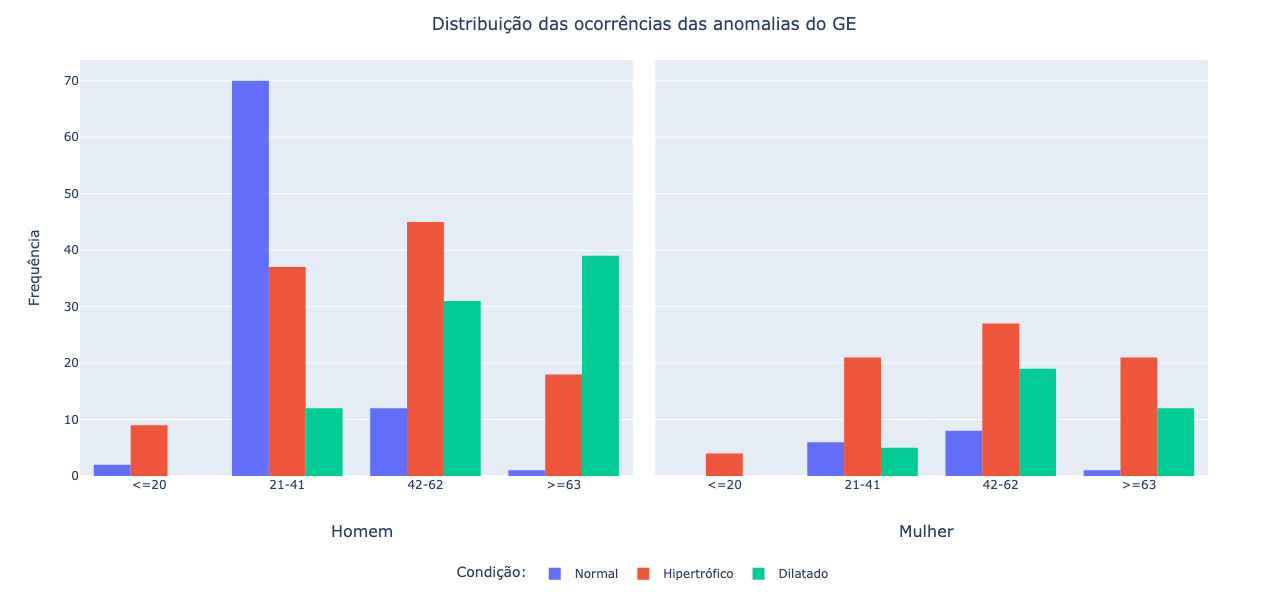
\includegraphics[width=1\textwidth]{figures/fig012.png}
    \caption*{Fonte: Autor}
    \label{fig:fig012}
\end{figure}

%---------------------------------------------------------
\section{Pré-Processamento}
\label{subsec:cap4_preprocess}

Na fase de pré-processamento será utilizado o conjunto de dados \gls{ACDC}. No \gls{ACDC} será separado aplicado três classe: \gls{CMH} do grupo HCM, \gls{CMD} do grupo HCM e NOR para os demais grupos. O conjuntos de \textit{frames} utilizados serão os definidos na fase diastólica e a quantidade de \textit{frames} é variada para cada paciente. As características radiômicas e profundas serão extraídas e posteriormente, será aplicado o \textit{F-Test} para selecionar as características mais relevantes, mantendo o mesmo número de ambas as partes. Por fim este resultado será concatenado e servirá de entrada para a rede proposta de autoatenção.

%---------------------------------------------------------
\section{Extração de Características Radiômicas}
\label{subsec:cap4_features_radiomicas}

Serão extraídas características radiômicas de fase diastólica, representada por um conjunto de fatias variando entre 6 e 18 \textit{frames}, de cada paciente usando \gls{GLCM} e estatísticas baseadas em histograma. Será aplicado o filtro \gls{LoG} com cinco valores diferentes em cada parte para suavizar as imagens e realçar as bordas. Foi calculado características \gls{GLCM} como contraste, entropia, correlação, homogeneidade e energia para cada filtro \gls{LoG}. Também é calculado características de intensidade como média, variância, média dos percentis (10 e 90), desvio robusto da média absoluta, curtose e assimetria usando estatísticas de primeira ordem. Foram obtidos 78 características radiômicas para cada paciente dentro da quantidade de fatias extraídas na fase diastólica.

%---------------------------------------------------------
\section{Extração de Características Profundas}
\label{subsec:cap4_features_profundas}
 
Para extrair características profundas das imagens de \gls{RMC}, é utilizada a arquitetura pré-treinada de um \textit{ResNet50} sem sua última camada totalmente conectada, treinada no conjunto de dados \textit{ImageNet}. Estudos anteriores demonstraram que o pré-treinamento com \textit{ImageNet} pode melhorar o desempenho de tarefas de classificação de imagens médicas. \textit{ResNet50} é um modelo de rede neural convolucional profunda com 50 camadas que compreende muitos blocos residuais. Cada bloco contém módulos de convolução e uma conexão de salto que transfere a informação do bloco anterior para o próximo bloco. A conexão de salto ajuda a reter a informação semântica mais básica aprendida nas camadas anteriores, que de outra forma se tornaria abstrata devido à conexão de longa cadeia. A conexão de salto também evita o desaparecimento do gradiente nas camadas mais profundas ao fornecer um caminho alternativo para a retropropagação. A informação da conexão de salto é adicionada à informação calculada em cada bloco \cite{aiSelfAttentionBasedFusion2023}. Ao todo são 2048 características coletadas da saída deste modelo.

%---------------------------------------------------------
\section{Concatenação}
\label{subsec:cap4_unificando_features}

Um vez em posse das features radiômicas, é aplicado um \textit{F-Test} tanto às 78 características radiômicas quanto às 2048 características profundas, reduzindo cada um dos vetores ao espaço de 64 características. No método de fusão convencional, simplesmente é concatenado os dois vetores de características como na Eq. \ref{eq:concat}, onde \textit{Concat} simplesmente concatena os dois vetores. Unificando ambos os vetores obtemos o valor resultante de 128 características o qual será enviado ao mecanismo de autoatenção.

\begin{equation}
F_{hd} = \textit{Concat}(F_h, F_d)
\label{eq:concat}
\end{equation}

%---------------------------------------------------------
\section{Modelo de Autoatenção}
\label{subsec:cap4_mod_self_attention}

Neste trabalho é empregado o mecanismo de autoatenção para aprender a importância de cada característica e capturar suas dependências de longo alcance. Como ilustrado na Figura \ref{fig:fig011}, o módulo de fusão de autoatenção é utilizado para mapear uma consulta ($Q$), chave ($K$) e valor ($V$) para um valor de atenção. São utilizadas as 128 características concatenadas $F_{hd}$ como \textit{tokens} e projetada cada característica em três matrizes aprendíveis: matriz chave $K$, matriz consulta $Q$ e matriz de valor $V$ por produto escalar com as matrizes $W_{Q}$, $W_{K}$ e $W_{V}$. Logo os valores $Q$, $K$, $V$ são denotados como $W_{Q}F_{gd}$, $W_{K}F_{gd}$, $W_{V}F_{gd}$ respectivamente, onde $W_{Q}$, $W_{K}$ e $W_{V}$ representam a transformação linear para as matrizes $Q$, $K$ e $V$. O módulo de fusão baseado em autoatenção é definido como segue na Equação \ref{eq:attention}, onde $d_{k}$ é a dimensão do valor de $K$. Sem utilizar operações recorrentes ou convolucionais, o módulo de fusão de autoatenção pode modelar as dependências de longo prazo entre as características de entrada.
Este módulo calcula de forma adaptativa os pesos entre as características com base em sua importância e relevância, capturando de forma mais abrangente as associações entre características radiômicas e profundas. Tal processo realça a capacidade expressiva das características fundidas e permite que o modelo foque mais precisamente nas características mais informativas para prever \gls{CMH} e reduzir a influência de características irrelevantes na previsão. Além disso, o modelo pode alocar dinamicamente atenção a diferentes amostras de imagens de \gls{RMC}. Essa flexibilidade permite com que o modelo se adapte melhor à representação de características de diferentes amostras, melhorando a precisão e a generalização da previsão.

A função de perda utilizada utilizada no modelo é a função de entropia cruzada binária, do termo  \gls{BCE}, que é calculada pela Equação. \ref{eq:bce} onde $\mathcal{L}_{bce}$ denota o \gls{BCE}, $N$ denota o número de imagens de \gls{RMC}, $r$ denota a classe alvo de \gls{CH} e $\hat{r}$ o valor previsto pelo modelo de \gls{CMH}, 1 indica indícios de \gls{CMH} e 0 sua ausência.

\begin{equation}
\mathcal{L}_{bce} = -\frac{1}{N} \sum_{i=1}^N
(r_i \ln \hat{r}_i + (1 - r_i) \ln (1 - \hat{r}_i))
\label{eq:bce}
\end{equation}

%---------------------------------------------------------
\section{Métricas}
\label{subsec:cap4_metrics}
Para medir o desempenho da solução serão aplicadas as seguintes métricas: acurácia, precisão, revocação expressas pelas equações \ref{eq:acc}, \ref{eq:precision} e \ref{eq:recall}.
Também é calculada a \gls{AUC}, também reconhecida como a área que avalia o modelo em diversos limites contínuos de decisão, verificando a taxa de verdadeiros positivos contra falsos positivos em cada limite.

\begin{equation}
  \textit{Acurácia} = \frac{\textit{TP} + \textit{TN}}{\textit{TP} + \textit{TN} + \textit{FP} + \textit{FN}}
  \label{eq:acc}
\end{equation}

\begin{equation}
  \textit{Precisão} = \frac{\textit{TP}}{\textit{TP} + \textit{FP}}
  \label{eq:precision}
\end{equation}

\begin{equation}
  \textit{Revocação} = \frac{\textit{TP}}{\textit{TP} + \textit{FN}}
  \label{eq:recall}
\end{equation}

%---------------------------------------------------------
\section{Arquitetura Proposta}
\label{subsec:cap4_architecture}

O esquemático da arquitetura proposta pode ser conferida na Figura \ref{fig:fig011}. A imagens de \gls{RMC} são expostas ao seletor de características via \textit{F-Test}, as características selecionadas são concatenadas e enviadas ao módulo de fusão de autoatenção, por fim uma camada linear de 128 características precede um camada linear com um único neurônio para a classificação binária. A arquitetura proposta tem como base o trabalho de \cite{aiSelfAttentionBasedFusion2023}.

\begin{figure}[htbp]
    \centering
    \caption{Arquitetura Proposta}
    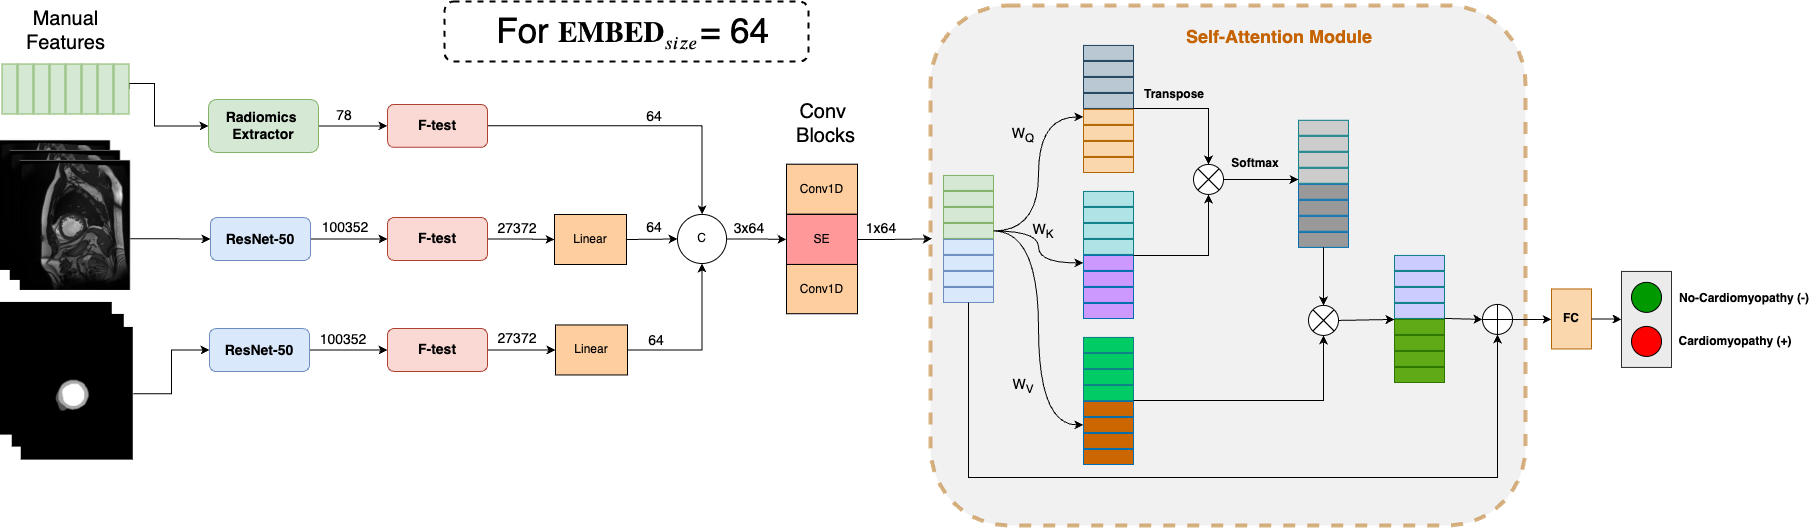
\includegraphics[width=1\textwidth]{figures/fig011.png}
    \caption*{Fonte: Autor}
    \label{fig:fig011}
\end{figure}

%---------------------------------------------------------
\section{Considerações Finais do Capítulo}
\label{sec:cap4_consideracoes_finais}

Como considerações, destacam-se o uso de base de dados pública, com dados de pacientes incluindo o conjuntos de fatias que identificam a ação de sístole e diástole do coração. É aplicado pré-processamento do qual é extraído manualmente 78 características radiômicas, características estas que analisam textura, níveis e variações dos tons de cinza incluindo diversas estatísticas como de primeira ordem e o \gls{GLCM}. Ainda em fase de pré-processamento é extraída as características profundas oriundas do modelo de visão \textit{ResNet50}, com os pesos treinados na base de dados da \textit{ImageNet}. É removida a última camada linear da \textit{ResNet50} resultando ao seu final, sem a camada classificadora, 2048 características. Em posse de ambas as features, é aplicada a técnica de \textit{F-Test} para obter as 64 características mais relevantes e, após, concatená-las obtendo um vetor de características de 128 características. Este vetor é exposto ao módulo de fusão com autoatenção, identificando as características mais determinantes independente de espacialidade. 